\section{Specifikacije za izršavanje}

Kako bi se hardver efikasno projektovao i particionisao potrebno je početi od
softverske implementacije na višem nivou apstrakcije.  \\
Jezici visokog nivoa kao što je Python su veoma dobri za ovu namenu.

\begin{figure}[h]
  \centering
  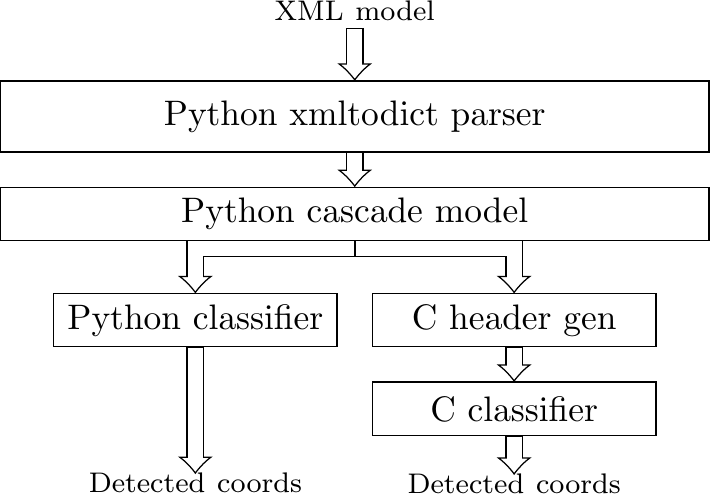
\includegraphics[width=0.9\textwidth]{bdp/sw_arch/sw_arch1.png}
  \caption{Veza Python modela sa XML modelom i C specifikacijom}
  \label{sw_arch_spec1}
\end{figure}

Na slici(\ref{sw_arch_spec1}) prikazana je struktura koda u slučaju Python i C
klasifikatora. \\

\noindent
Na ulazu se nalazi XML model dobijen treningom pomoću OpenCV opisan u sekciji
\ref{opencv_model}. \\
Kao jezik za parsiranje XML fajla se koristi Python.
Zbog velikog broja Python paketa dostupnih sa gotovim rešenjima za većinu softverskih problema, problem
parsiranja XML fajla se može rešiti korišćenjem paketa xmltodict\footnote{\url{https://pypi.org/project/xmltodict/}}. \\
\emph{Xmltodict} parsira XML fajl i skladišti ga u Python dictionary. \\
Klase \emph{CascadeClass}, \emph{StageClass}, \emph{FeatureClass} i
\emph{RectClass}  \footnote{\texttt{\detokenize{cascade_classifier/python_model/cascade.py}}} napisane u Pythonu
predstavljaju Python model kaskadnog klasifikatora. \\

Napisan je i Python specifikacija za isvršavanje koja direktno koristi Python
klase za detekciju objekata. \\
Veza između Python modela i C specifikacije realizovana je preko \emph{C Header}
fajla koji je generisan pomoću Python-a.